% !TEX root = ../main.tex

O documento de casos de uso tem como finalidade o detalhamento a fundo dos recursos do programa, aqui chamados de caso de uso, listados na Seção \ref{subsub:recursos_produto} deste documento, colocando todas as suas características, restrições e caminhos possíveis.

\subsection{Identificação dos atores}

Neste contexto, atores são representações genéricas de usuários do sistema, podendo ser qualquer utilizador, sem se preocupar com nome do executor, apenas com sua função, esses atores estão listados na Tabela \ref{tab:atores}.

\begin{table}[H]
\centering
\begin{tabular}{|l|p{8cm}|}

\hline
\textbf{Atores} &
\textbf{Descrição}
\\ \hline
%----------------------------------------------
Engenheiro de Requisitos &
Responsável, em metodologias tradicionais, pela elicitação dos requisitos, pela manutenção da rastreabilidade do sistema e gerência dos requisitos.
\\ \hline
%----------------------------------------------
Equipe de portfólio &
Responsável, em metodologias ágeis, por gerir a parte do portfólio, como temas de investimento e épicos.
\\ \hline
%----------------------------------------------
Equipe de programa &
Responsável, em metodologias ágeis, por gerir as features do sistema e manter a entrega das releases em dia.
\\ \hline
%----------------------------------------------
Time &
Responsável, em metodologias ágeis, por implementar as histórias de usuário.
\\ \hline

\end{tabular}
\caption{Atores do sistema}
\label{tab:atores}
\end{table}

\subsection{Diagrama de casos de uso}

Uma forma de apresentar os recursos do sistema de forma clara e objetiva é com a utilização de Diagramas de Casos de Uso, os quais apresentam todos os Casos de Uso e quais suas interações com os atores. Com a utilização deste diagrama, pode-se obter o entendimento sobre o que cada ator poderá fazer ao utilizar a ferramenta.

O diagrama está representado nas Figuras \ref{img:DiagramaUC1}, \ref{img:DiagramaUC2} e \ref{img:DiagramaUC3} referentes às abordagens tradicional, ágil, e à definição de metodologia, respectivamente:

\subsubsection{Parte 1: Definição da metodologia e processos híbridos}
	Na primeira parte do diagrama de casos de uso, presente na Figura \ref{img:DiagramaUC1}, estão representadas as relações dos atores \textbf{engenheiro de requisitos} e \textbf{equipe de portfólio} com o caso de uso \textbf{UC1.3.1.1 - Definir Metodologia} e de todos os atores com os casos de uso da característica \textbf{C1.4.1 - Criar processos Híbridos}, referente à metodologias híbridas.
	\\
\begin{figure}[H]
	\centering
	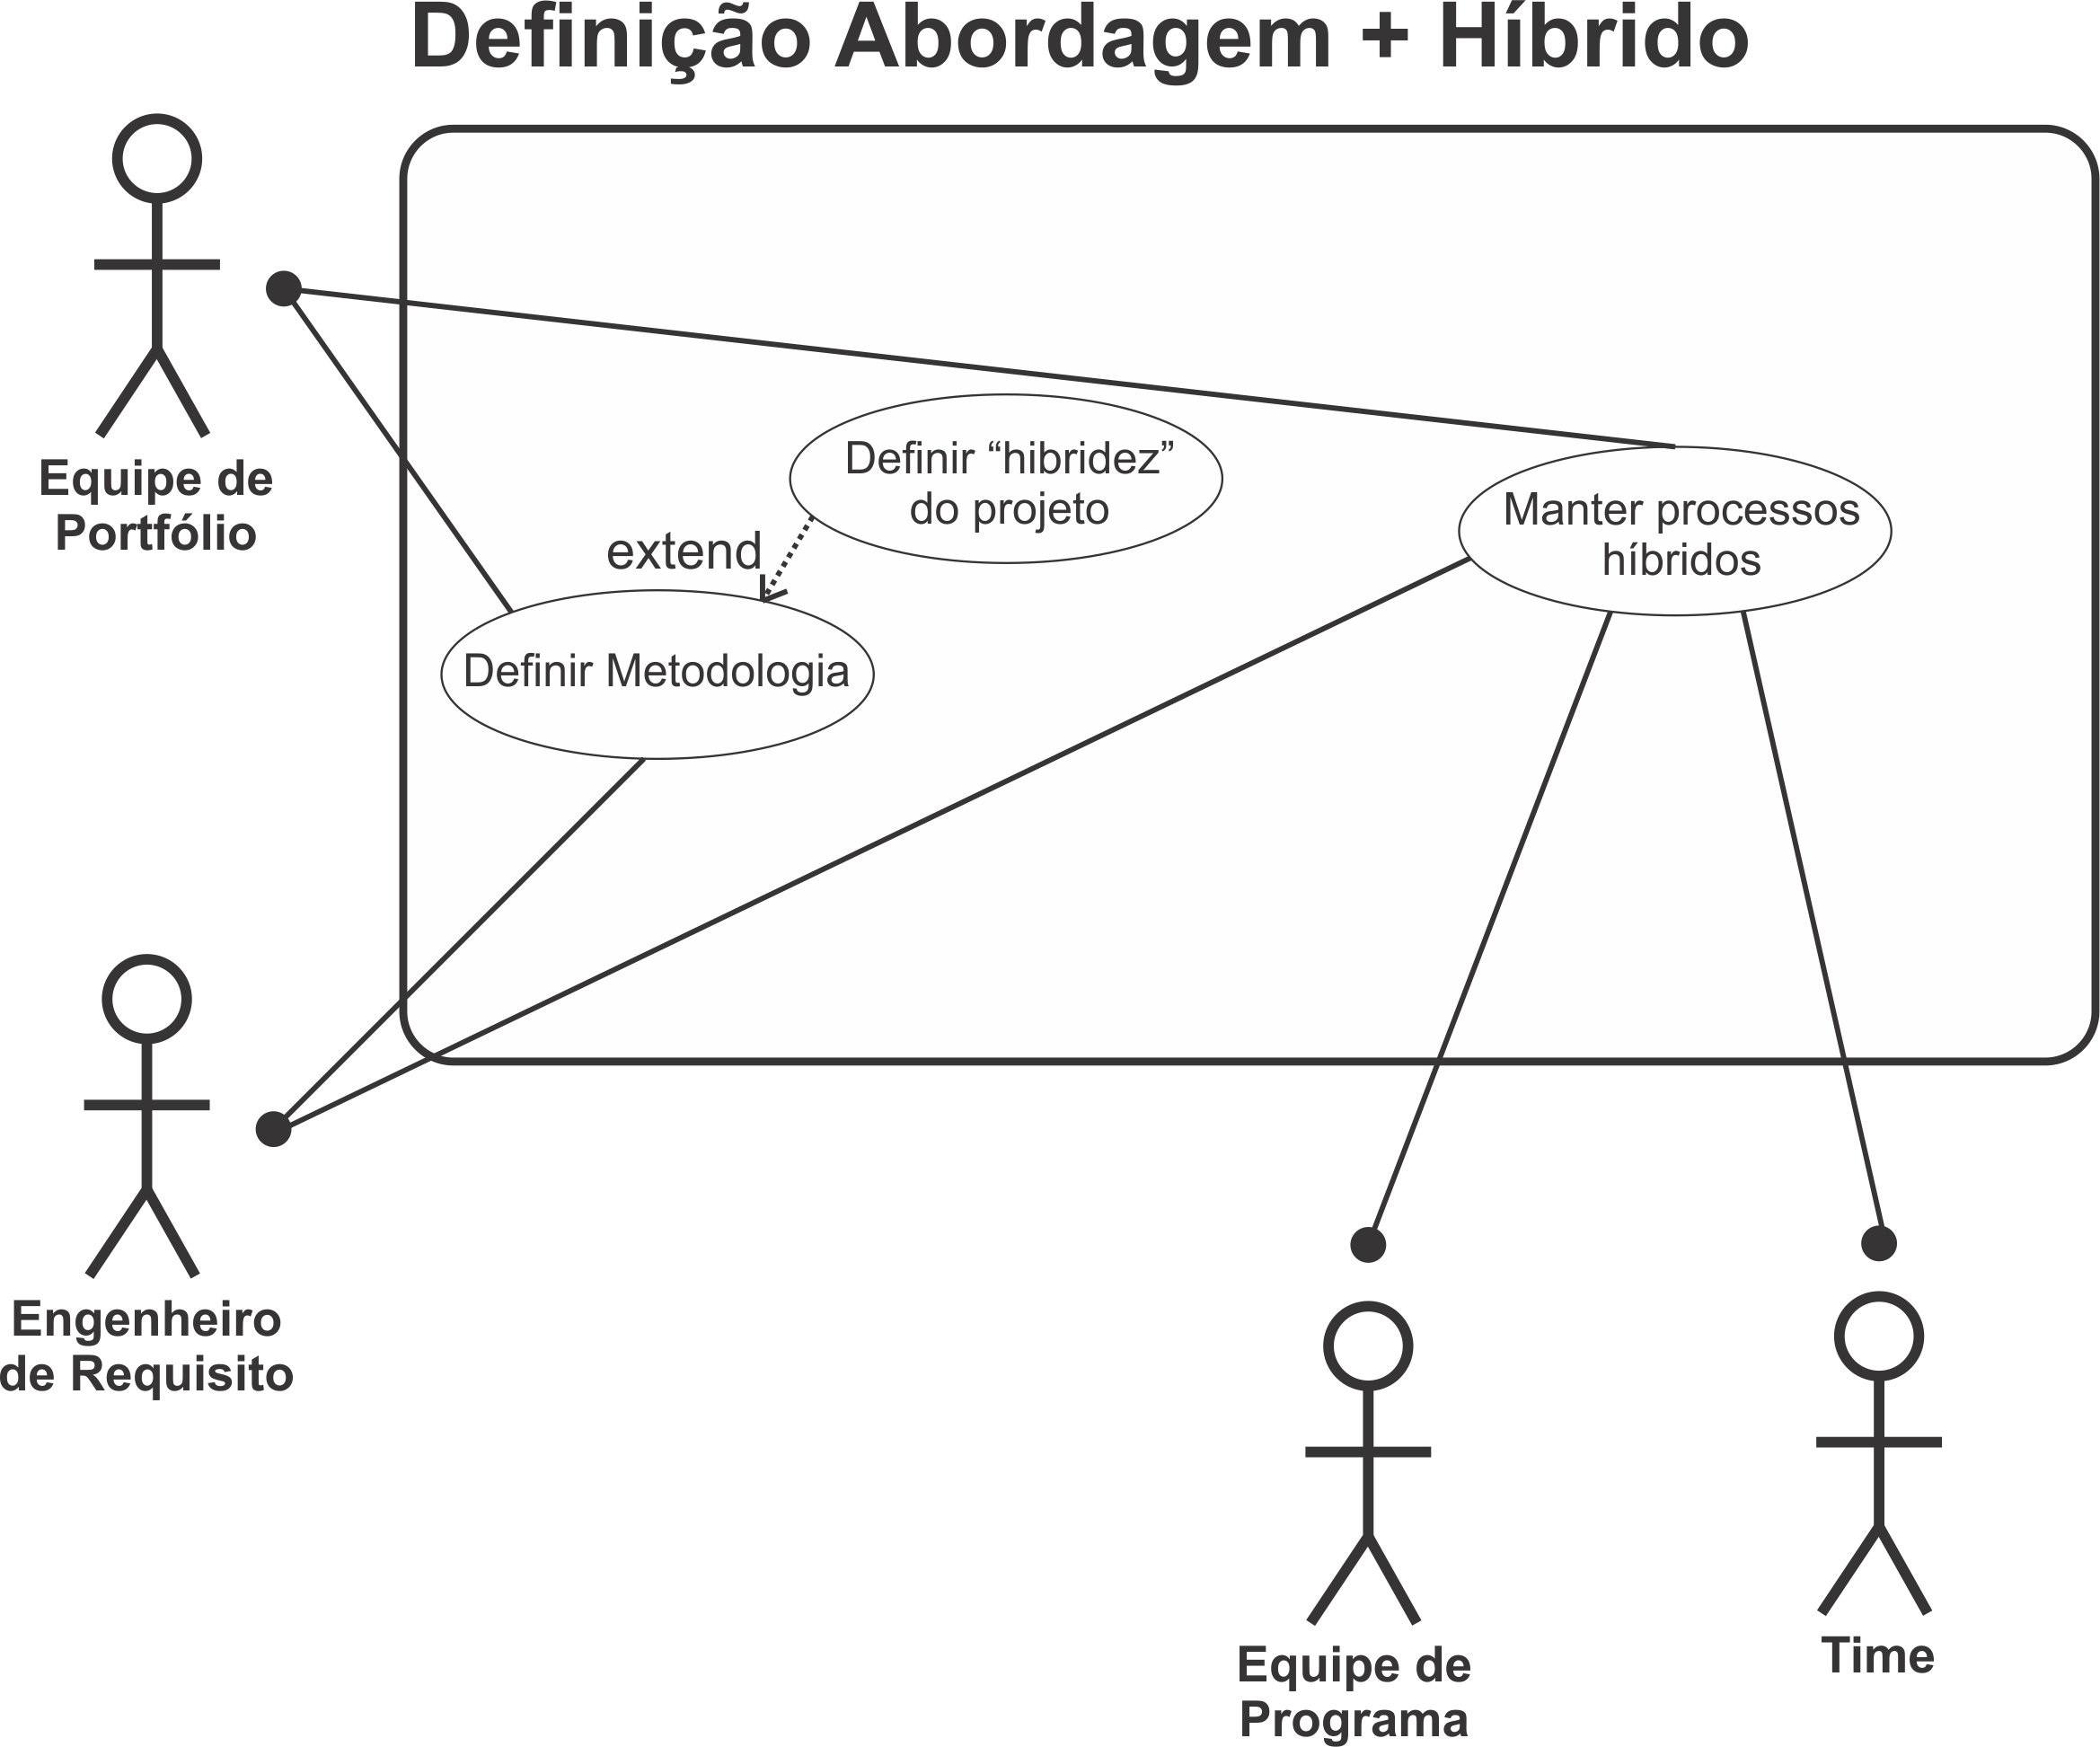
\includegraphics[width=0.8\textwidth]{imgModelagem/DiagramaUC1}
	\caption{Diagrama de casos de uso 1: Definição da metodologia e processos hibridos}
	\label{img:DiagramaUC1}
\end{figure}

\subsubsection{Parte 2: Abordagem Tradicional}

	Na segunda parte do diagrama de casos de uso, presente na Figura \ref{img:DiagramaUC2}, estão representadas as relações dos casos de uso referentes à metodologia tradicional com o ator \textbf{engenheiro de requisitos}.

\begin{figure}[H]
	\centering
	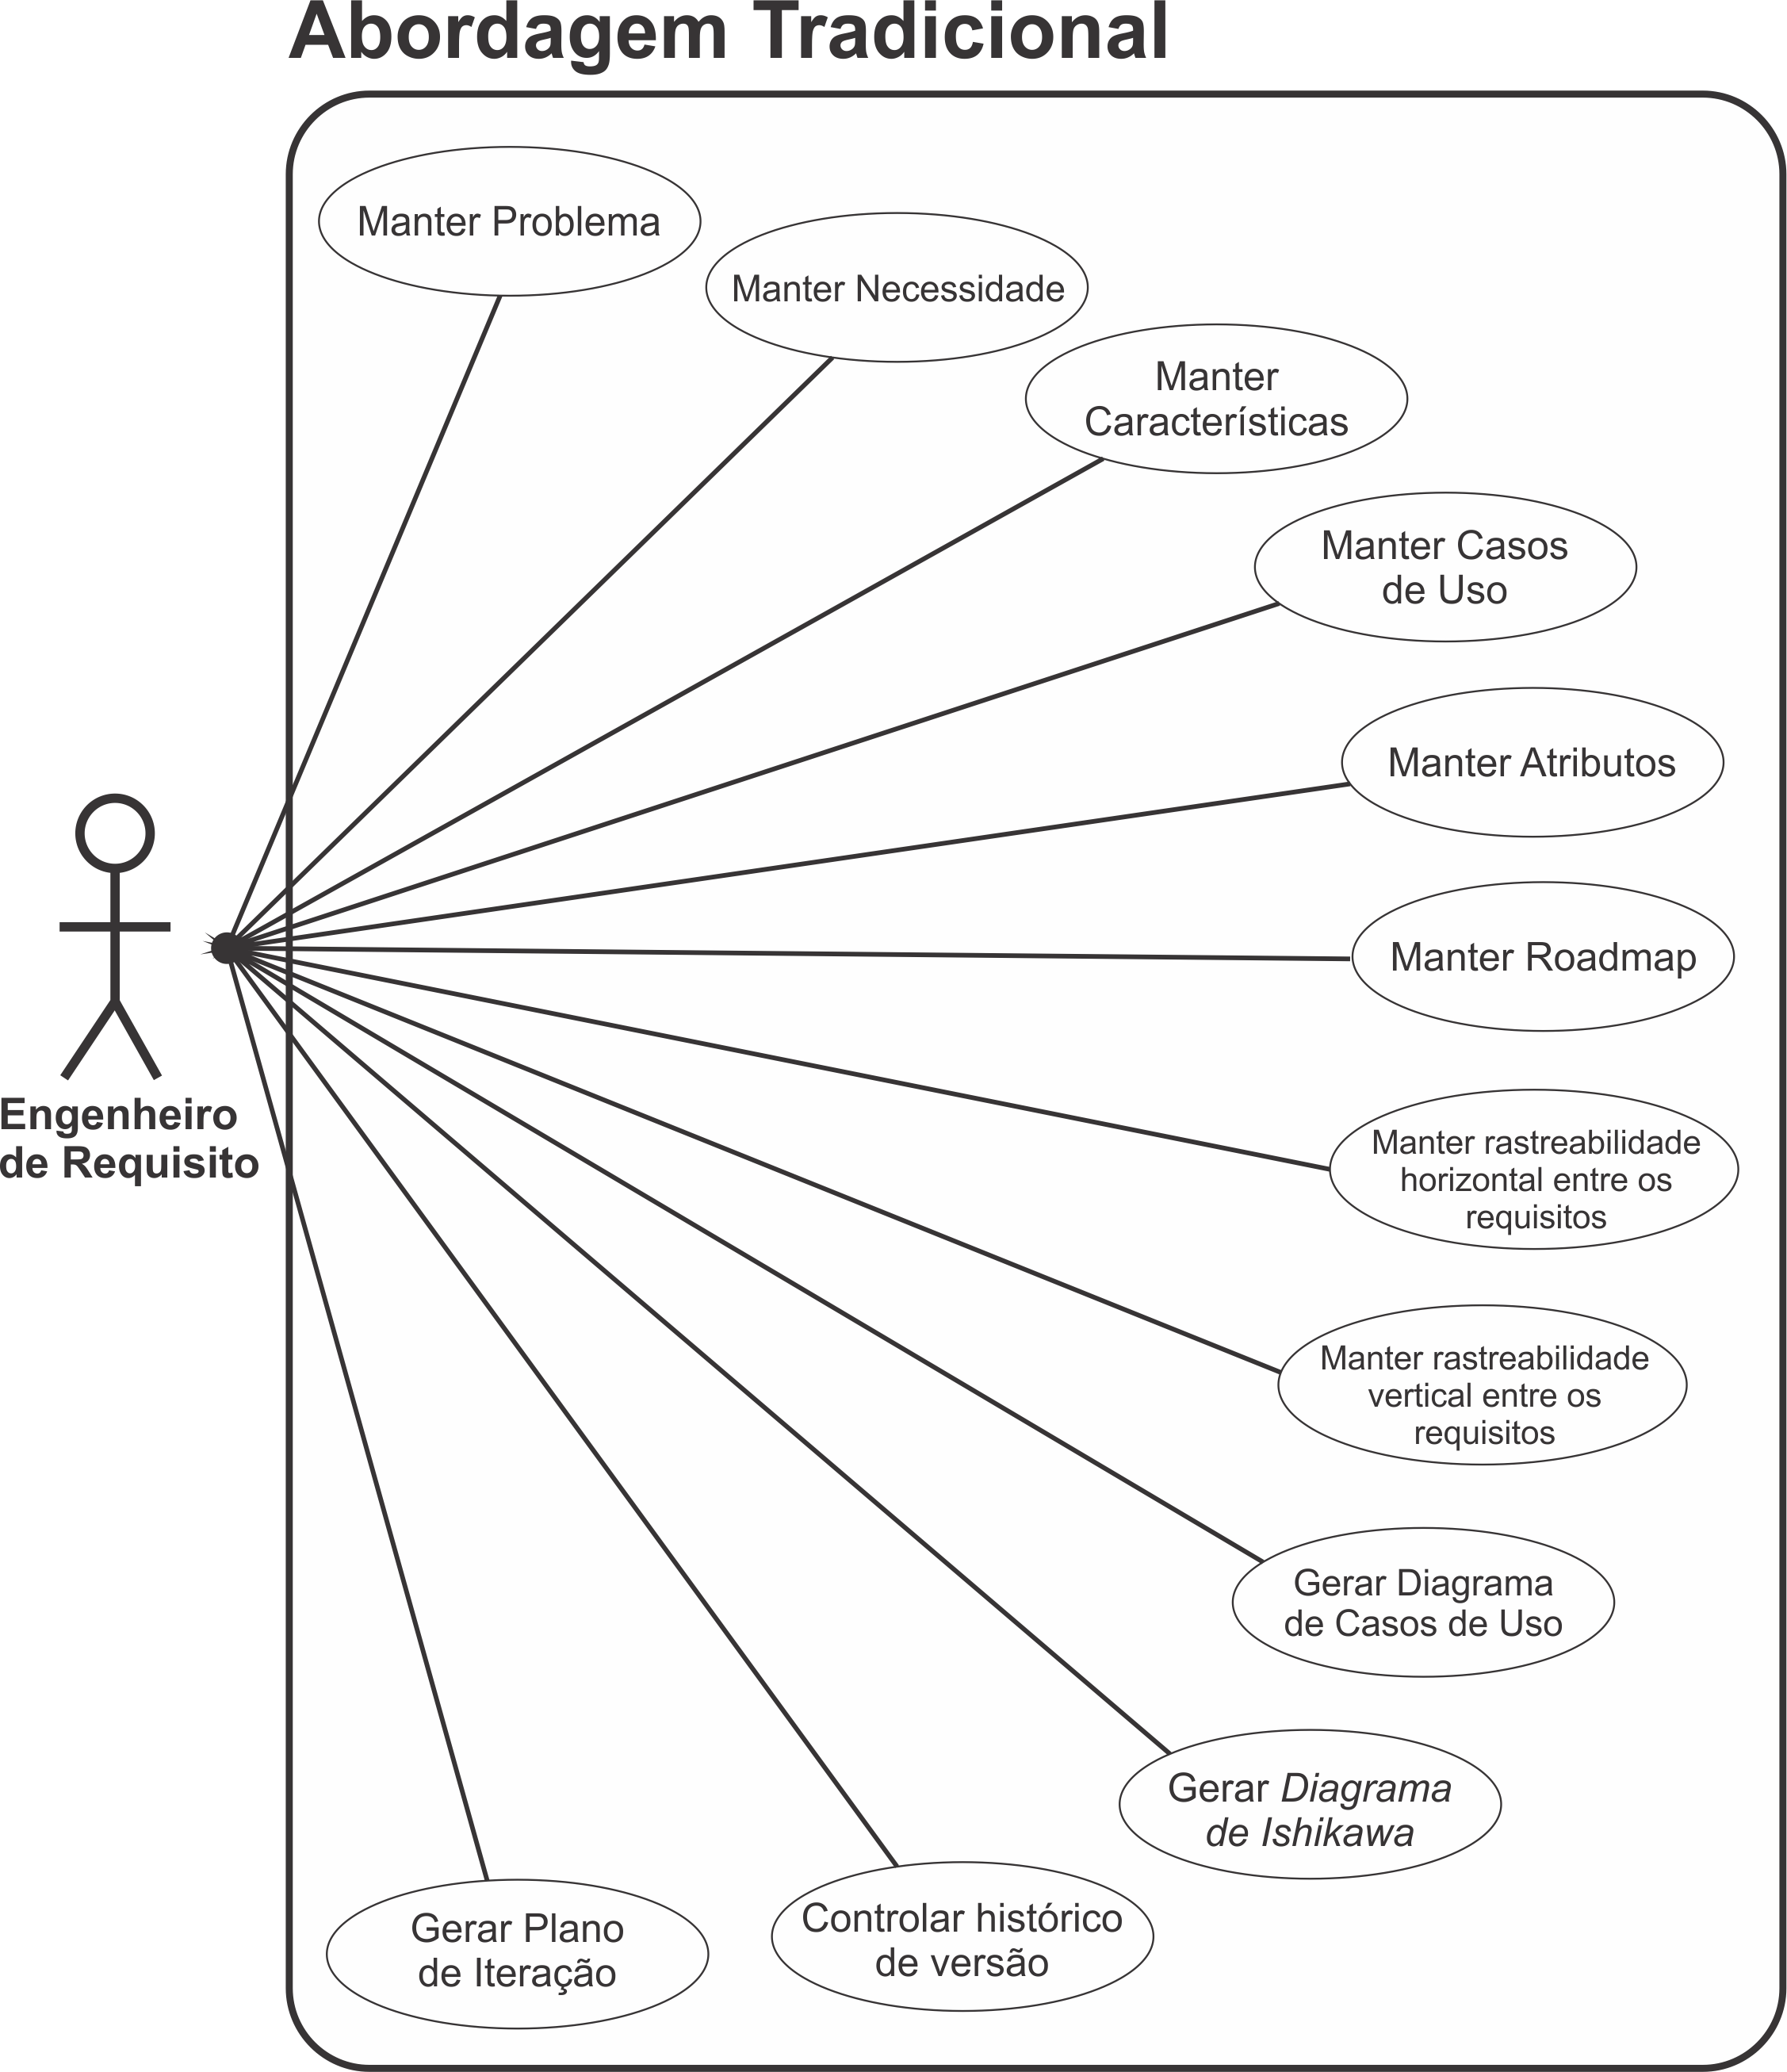
\includegraphics[width=0.8\textwidth]{imgModelagem/DiagramaUC2}
	\caption{Diagrama de casos de uso 2: Abordagem Tradicional}
	\label{img:DiagramaUC2}
\end{figure}

\subsubsection{Parte 3: Abordagem Ágil}
	Finalmente na terceira parte do diagrama de caso de uso, presente na Figura \ref{img:DiagramaUC3}, estão representadas as relações dos casos de uso referentes à metodologia ágil com os atores \textbf{equipe de portfólio}, \textbf{equipe de projeto} e \textbf{equipe de time}.

\begin{figure}[H]
	\centering
	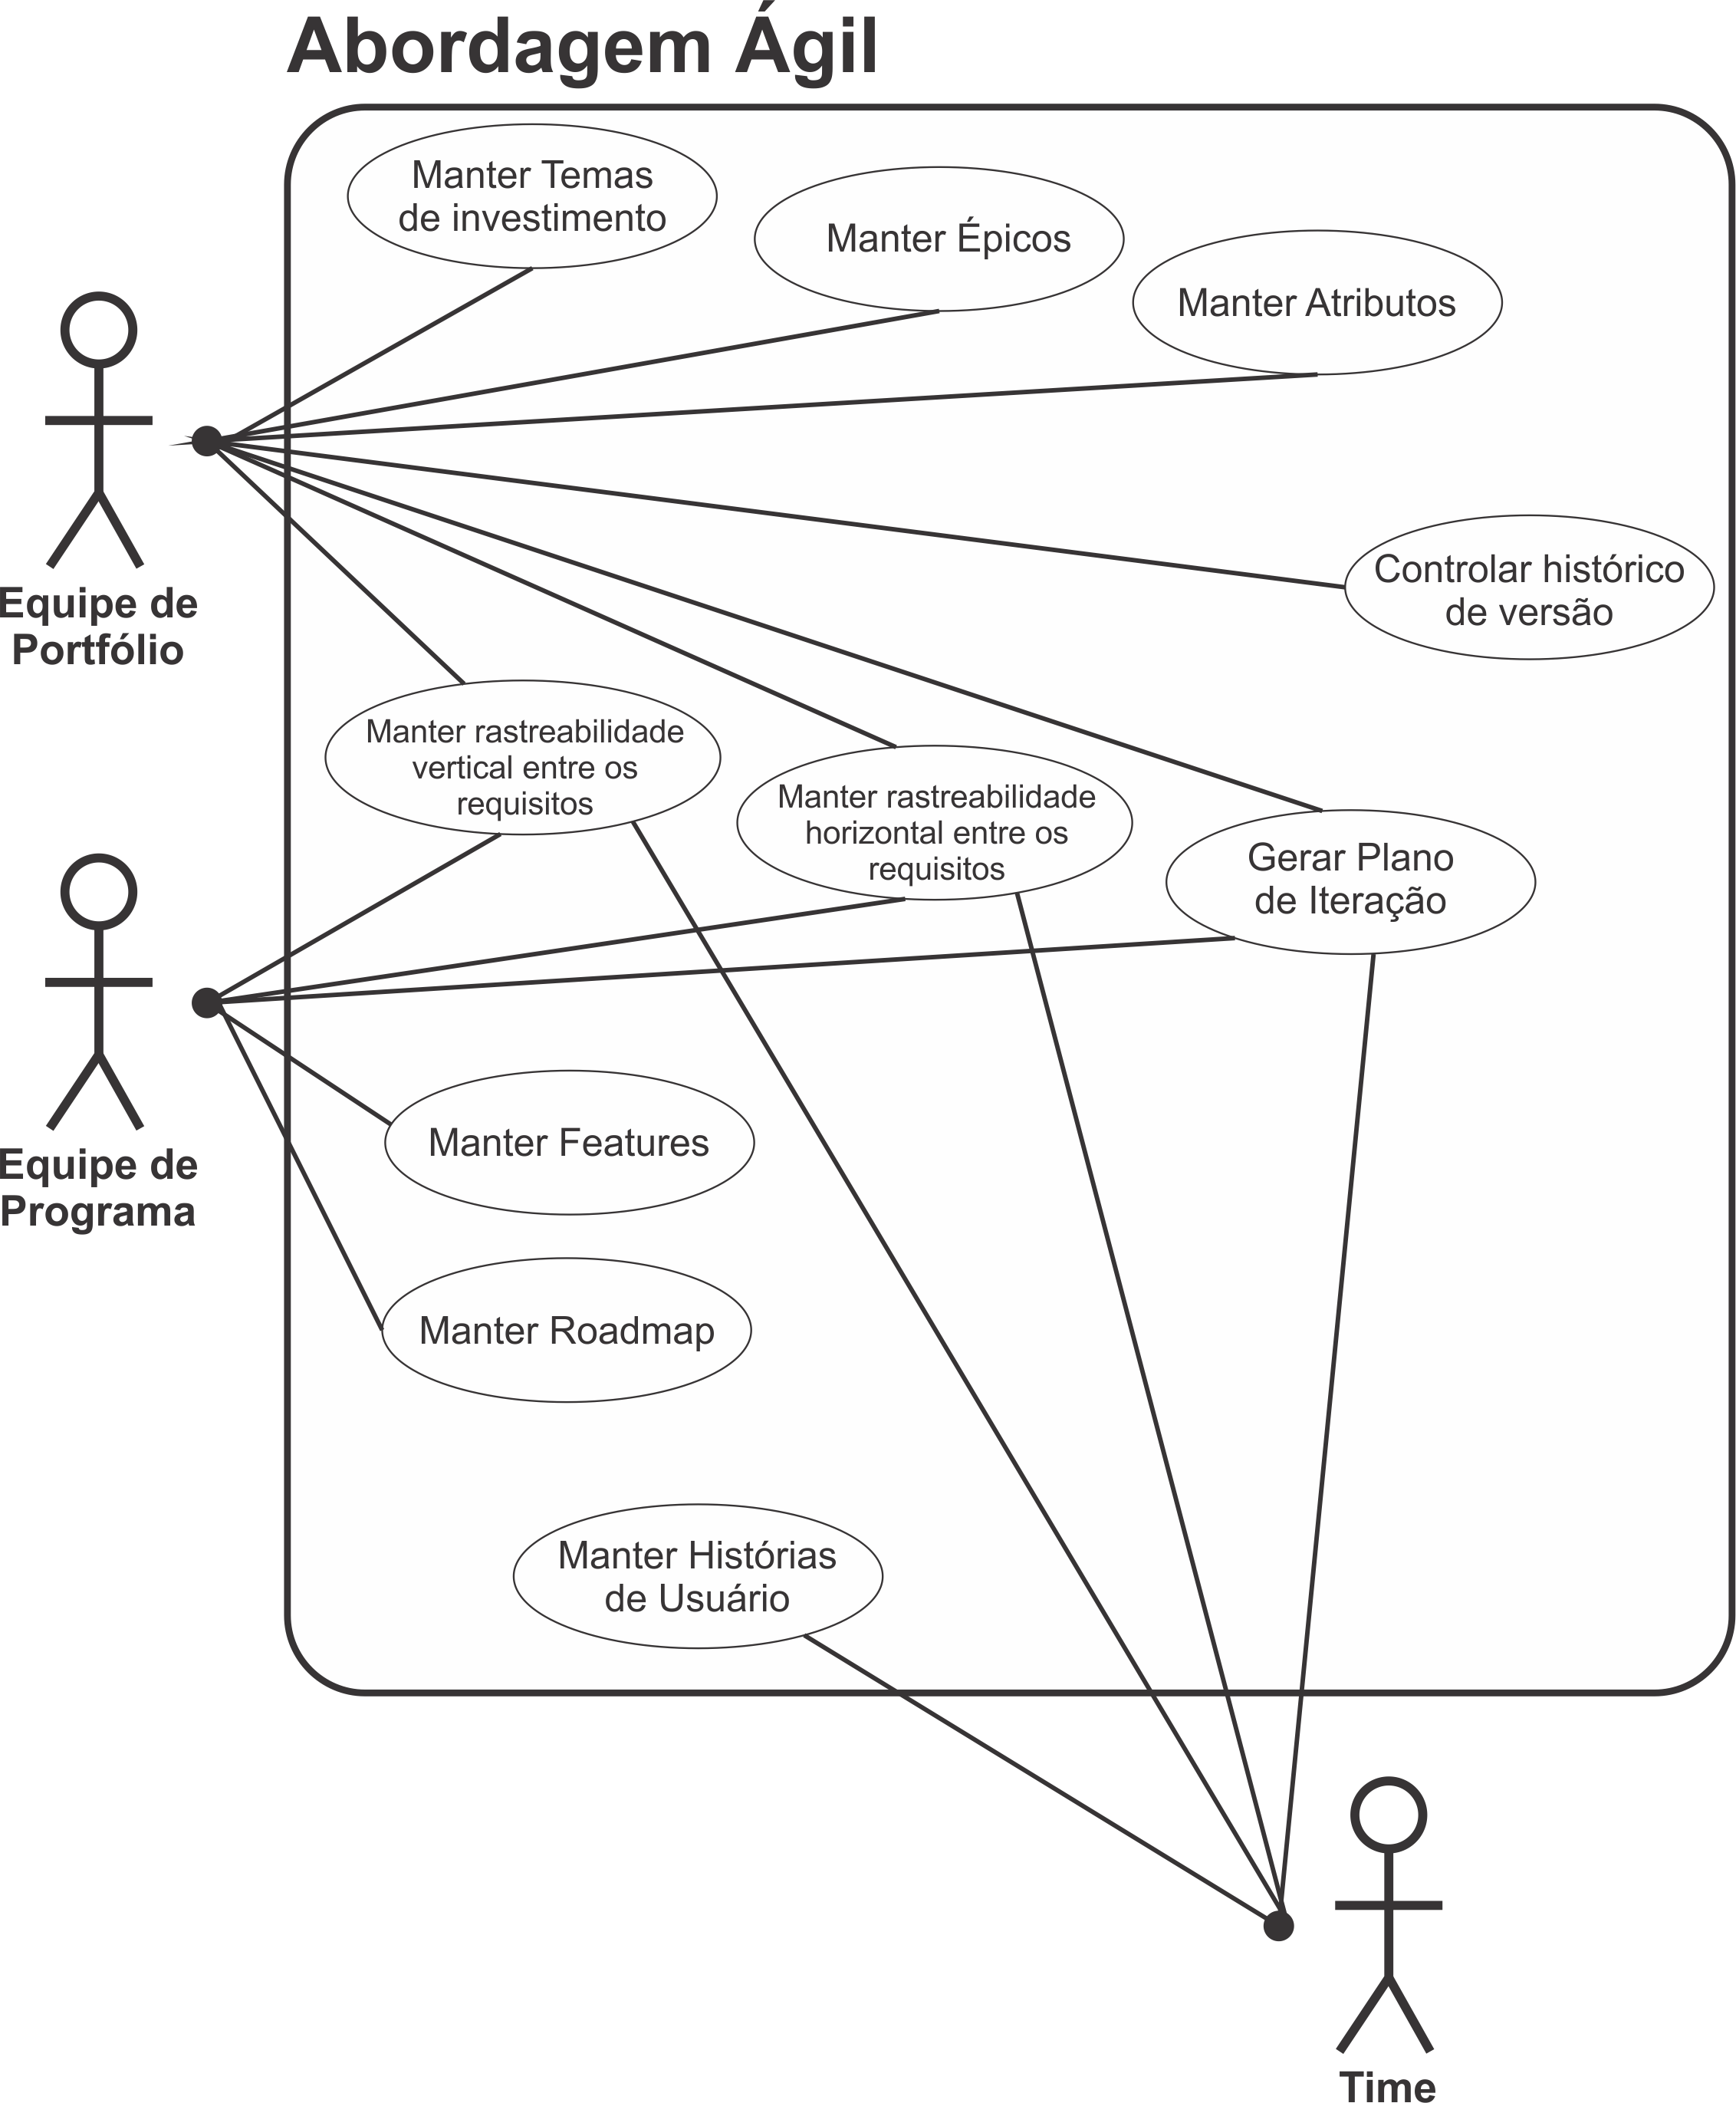
\includegraphics[width=0.8\textwidth]{imgModelagem/DiagramaUC3}
	\caption{Diagrama de casos de uso 3: Abordagem Ágil}
	\label{img:DiagramaUC3}
\end{figure}
%-------------------------------------FISHBONE AQUI----------------------------------------

\subsection{Detalhamento dos casos de uso}

Detalhamentos de casos de uso servem para definir o que cada caso de uso fará, quem irá realizá-lo, e como ele irá responder a falhas caso haja, e todos os seus caminhos possíveis.

A seguir está o detalhamento do caso de uso que será implementados na sprints 1, detalhada na Tabela \ref{tab:primeiro_roadmap}.

\subsubsection{Caso de Uso - UC1.3.1.1 - Definir Metodologia}

\paragraph{Descrição:}

Este caso de uso especifica a ação do sistema de, dada as informações solicitadas, selecionar a melhor rota possível para o desenvolvimento do projeto, podendo o usuário, ao final do questionário, decidir se irá seguir ou não a rota sugerida, e então preparar a ferramenta para a metodologia escolhida.

\begin{enumerate}
	\item \textbf{Atores:}
		Engenheiro de requisitos, Equipe de portfólio. 
	\item \textbf{Pré-condições:}
		Não existe pré condições para este caso de uso.
	\item \textbf{Pós-condições:}
		A rota a ser utilizada deve estar definida ao final da execução deste caso de uso.
	\item \textbf{Requisitos Funcionais:}
		\begin{itemize}
			\item \textbf{RF049} - Fazer relatório com perguntas específicas para definir características do processo;
			\item \textbf{RF050} - Definir em qual metodologia o processo do cliente se encaixa;
		\end{itemize}
	\item \textbf{Requisitos Não Funcionais:}
		\begin{itemize}
			\item RNF01 - O usuário não deve necessitar de treinamento para utilizar a ferramenta;
			\item RNF02 - O usuário não deve levar mais de um mês para estar produtivo na utilização da ferramenta (não demorar mais de cinco segundos para encontrar a proxima funcionalidade desejada).
			\item RNF07 - O sistema deve ter um tempo de resposta em qualquer página de no máximo dois segundos e em média um segundo;
			\item RNF08 - O sistema deve ter no máximo 1 consulta ao banco de dados por funcionalidade;
		\end{itemize}
\end{enumerate}

\paragraph{Fluxo básico}

	\begin{enumerate}
		\item Ator decide criar um novo projeto;
		\item Sistema apresenta um questionário para recolher informações do projeto, presente na seção \ref{sec:perguntas_do_questinario};
		\item Ator responde questionário;
		\item Sistema calcula estatisticamente qual rota deve ser utilizada, de acorodo com as respostas do ator, selecionando as rotas de cada pergunta respondida de acordo com qual metodologia elas pertencem;
			\label{item:1.3.1.1_empate}
		\item Sistema apresenta ao ator a escolha da metodologia;
		\item Usuário aceita a metodologia;
			\label{item:1.3.1.1_recusado}
		\item Sistema prepara a ferramenta para utilização da metodologia escolhida.
			\label{item:1.3.1.1_retorno1}
	\end{enumerate}

\paragraph{Fluxo alternativo A}

	\begin{enumerate}
		\item No passo \ref{item:1.3.1.1_empate} do fluxo básico, caso haja um empate entre metodologias;
		\item Sistema apresenta ao ator as metodologias empatadas e suas características;
		\item Ator escolhe a metodologia que deseja;
		\item O fluxo retorna para o passo \ref{item:1.3.1.1_retorno1} do fluxo básico.
	\end{enumerate}

\paragraph{Fluxo alternativo B}

	\begin{itemize}
		\item No passo \ref{item:1.3.1.1_recusado} do fluxo básico, caso o ator não aceite a metodologia proposta pelo sistema;
		\item Ator rejeita a opção da metodologia escolhida pelo sistema;
		\item Sistema apresenta todas as opções de metodologias cadastradas para que o usuário possa escolher;
		\item retorna para o passo \ref{item:1.3.1.1_retorno1} do fluxo básico.
	\end{itemize}

\paragraph{Perguntas do questionário}
\label{sec:perguntas_do_questinario}
\clearpage
	\begin{longtable}{|p{3.5cm}|p{3.5cm}|p{3.5cm}|p{3.5cm}|p{2cm}|}
		\hline
		%--------------------------
		\textbf{Pergunta} &
		\textbf{Práticas tradicionais} &
		\textbf{Práticas ágeis} &
		\textbf{Observações} &
		\textbf{Tipo da pergunta}
		\\ \hline
		\endhead

		\hline \multicolumn{5}{|r|}{\longtableendfoot} \\ \hline
		\endfoot

		% \hline
		\endlastfoot
		%--------------------------

		A equipe de desenvolivemnto irá mudar durante o projeto? &
		Requisitos tradicionais, problema, necessidade característica, requisitos funcionais e casos de uso. &
		Requisitos ágeis, tema de investimento, épicos, features e histórias de usuário. &
		Em casos no qual a equipe vai mudar durante o projeto, as metodologias ágeis falham em manter a documentação necessária para novos membros se atualizarem de como anda o projeto. &
		Equipe
		\\ \hline

		%-------------------------
		Seu cliente estará presente regularmente durante o projeto e ajudando constantemente em elicitar requisitos? &
		Equipe de desenvolvimento escreve todos os requisitos no início do projeto. &
		Cliente escreve os requisitos a medida em que o projeto avança. &
		Em casos no qual o cliente não pode estar presente constantemente no projeto, abordagens ágeis podem vir a ser falhas por haver dificuldades em elicitar requisitos novos e de priorizar os já elicitados. &
		Equipe
		\\ \hline

		%--------------------------
		A equipe de desenvolvimento é bem entrosada? &
		\begin{itemize}
			\item Processo engessado, sem possibilidades de alterações.
			\item Gerente atribuindo tarefas.
		\end{itemize} &
		\begin{itemize}
			\item Processo mais livre, baseado em testes feitos pela equipe e reuniões diárias.
			\item Membros da equipe podendo escolher quais tarefas fazer, uma vez que as mesmas estejam no escopo da sprint.
		\end{itemize} &
		Metodologia ágeis requerem uma equipe auto gerenciável e esteja bem entrosada evitando assim retrabalhos por falta de comunicação. &
		Equipe
		\\ \hline
		%----------------------------
		Sua equipe responde rápido a mudanças? &
		Requisitos definidos por contrato. &
		Requisitos abertos a alterações pelo cliente. &
		Metodologias ágeis, sofrerem muitas mudanças em seus requisitos, necessitam uma equipe que tenha capacidade de reagir rapidamente a alterações de escopo. &
		Equipe
		\\ \hline

		%---------------------------
		Sua equipe de desenvolvimento é experiente? &
		Nenhuma prática associada. &
		Codificação em pares. &
		Equipes mais experientes tendem a se adaptar e produzir melhor em metodologias ágeis pois geralmente eles acabam se tornando auto gerenciaveis e acabam por ter menos dificuldades tanto no relacionamento como na divisão e execução das tarefas. &
		Equipe
		\\ \hline
		%--------------------------

		Seu cliente exige muita documentação? &
		Documentação acima de código pronto. &
		Código acima de documentação &
		Metodologias tradicionais tendem a ter mais documentação que em metodologias ágeis, dependendo do projeto pode ser tanto uma vantagem como uma desvantagem. &
		Processo.
		\\ \hline 
		%-------------------------

		Seu cliente exige entregas contínuas de software? &
		Iterações longas com muita coisa para entregar. &
		Sprints de uma a quatro semanas com poucas funcionalidades para entrega porém com valor. &
		Em projetos tradicionais as entregas são mais espaçadas do que em projetos ágeis considerando a menor quantidade de reuniões disponíveis com o cliente. &
		Processo.
		\\ \hline
		%-----------------------

		Seu projeto é crítico? &
		Métodos formais. &
		Nenhuma prática associada &
		Projetos críticos requerem uma documentação formal com precisão, o que é algo mais simples de se alcaçar em metodologias tradicionais. &
		Processo.
		\\ \hline
		%------------------------

		Os requisitos do projeto mudarão constantemente? &
		Detalhamento de todos os requisitos no início do projeto. &
		Apenas detalhar requisitos no momento de implementá-los. &
		Projetos com mudaças intensas nos requisitos, geralmente tendem a ser projetos ágeis. &
		Negócio
		\\ \hline
	\caption{Perguntas para o projeto}
	\label{tab:perguntas_projeto}
	\end{longtable}